\documentclass{beamer}
\usepackage{pgfpages}
\usepackage{algorithm2e}
\usepackage{complexity}

\usetheme{Pittsburgh}
\useinnertheme{rectangles}
\usefonttheme{serif}
\newcommand{\T}{\mathcal{T}}

\newcommand{\tup}[1]
           {
             \relax\ifmmode
             \langle #1 \rangle
             \else $\langle$ #1 $\rangle$ \fi
           }

\title{\textbf{Product Constructions in Homological Quantum Codes}}
\subtitle{
ECE 621}


\author{\textbf{Edward Kim}}
% \date{\today}

\begin{document}
\begin{frame}
\titlepage
\end{frame}

\begin{frame}
  \frametitle{\textbf{Homological Quantum Codes}}
          \begin{enumerate}
            \item Homological Quantum Codes exploit homological invariants to perform quantum error correction.
            %To be more precise, 
              \item Various surface codes and their decoding schemes are examples of Homological Quantum Codes arising from tesselations of surfaces. 
              \item Several generalizations of these codes have been constructed through considering forms of \emph{homological products}.               
  
         \end{enumerate}
\end{frame}

\begin{frame}
    \frametitle{\textbf{Homology}}
    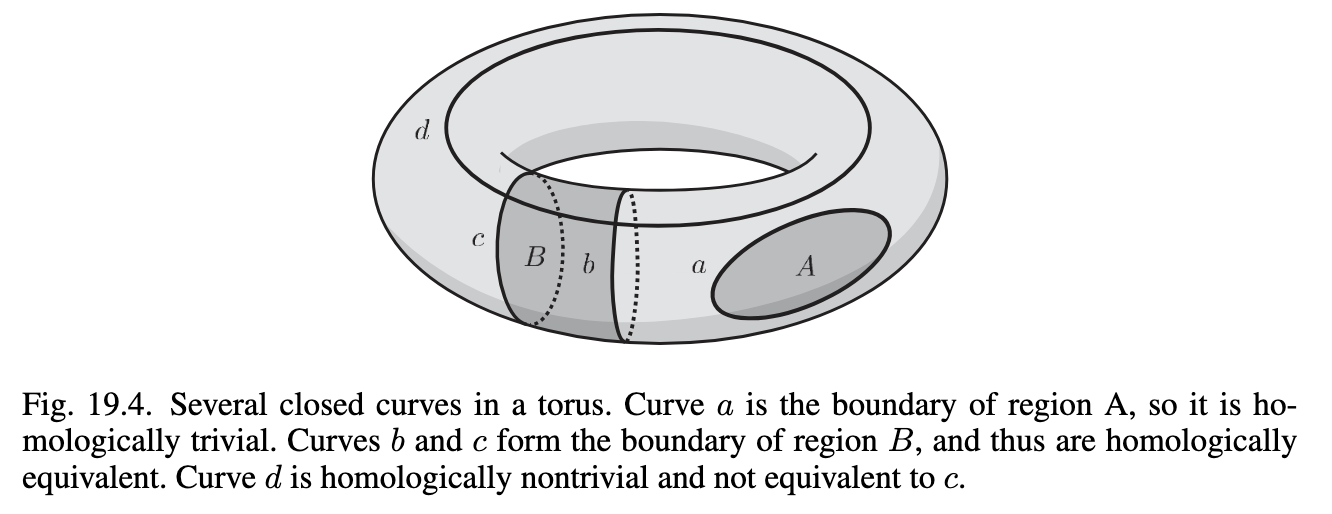
\includegraphics[scale=0.5 ]{torus}
\end{frame}

\begin{frame}
  \frametitle{\textbf{Product Constructions}}

\begin{enumerate}
  \item  The Tillich-Zémor hypergraph product constructs a $[[O(n_1n_2), k_1k_2 , \min\{d_1 , d_2\}]]$ quantum code from two classical $[n_i, k_i, d_i]$ codes 
  \item A closely-related construction was introducted by the Bravyi-Hastings' \emph{homological product codes}. These are "good" code families with stablizer weight $\leq 2\sqrt{n}$
\item Evra \textit{et. al} also considered a \emph{distance balancing method} which involves taking a product of a quantum code with a classical code. They showed that the tensor product of a $[[n, k, d_X , d_Z ]]$ quantum code with $r_X$ $X$-checks and a classical $[m, \ell, d]$ code
with $r$ checks begets a $[[nm + r_Xr, k\ell, d_X , d_Z d]]$ quantum
code.
\end{enumerate}
\end{frame}

\end{document}
